
\chapter{Analysis of Numerical Methods}
\label{chp:AnalNumMethod}
The most important property of a numerical method is convergence, because convergence guaranties that as we increase the spatial and temporal resolution of a numerical method, the numerical methods solutions better approximate the solutions of the differential equations. Which is precisely the desired property for a given  numerical method. For linear partial differential equations the Lax-equivalence theorem demonstrates that a numerical method is convergent if and only if it is stable and consistent []. Where consistency means that the error introduced by the numerical method at every time step approaches zero as the spatial and temporal resolution is increased. While stability means that the errors from all previous time steps are not amplified by the current time step.

The convergence of the finite difference volume methods and the finite element volume methods are inherited from the convergence of the finite volume methods at their core, which were shown to be convergent []. However, the convergence of the finite difference methods has not been shown for this particular equation and so we demonstrate that here. The consistency of the finite difference methods is very straightforward, given that we are using well tested approximations and so we instead focus on demonstrating stability for these methods. In particular we demonstrate von Nuemann stability [] for the linearised Serre equations. 

Having demonstrated the convergence of a particular method there are other properties that can be used to discriminate between two convergent numerical methods in order to pick the most appropriate numerical method for a particular differential equation. Such properties of numerical methods are: the order of accuracy and the computationally efficiency. For our methods we demonstrate the order of accuracy in [] using both analytical and forced solutions. 

The Serre equations can be written in conservation law form therefore their solutions conserve mass $h$, momentum $uh$, irrotationality $G$ [] and the Hamiltonian $\mathcal{H}$. The conservation of these quantities for the solutions of the numerical methods is investigated in chapter [].

The Serre equations are of particular interest for water wave modelling as they possess a dispersion relation that approximates the dispersion relation for the Euler equations well. Since the dispersion relation determines the speed of propagation for waves, approximating it well is of particular interest for tsunami modelling. Therefore knowing how well a given numerical methods dispersion relation approximates the dispersion relation of the Serre equations is an important question for our numerical methods as they are intended to be used for modelling tsunamis. For this reason we wish to know the error in the dispersion relation for all the numerical methods we are interested in; the finite difference volume methods and the finite element volume methods. 

In this chapter we will focus on analysing the stability and the dispersion relation of our numerical methods. We group these two analyses together as they employ very similar methods and require some working. We shall leave the rest of the analyses of the numerical methods in this thesis to chapters [] where we investigate the solutions of the numerical methods.

Both the dispersion relation and stability analysis are performed on the linearised Serre equation with horizontal beds. We neglect bed terms because our finite difference methods neglect them too and because the dispersion relation has no contribution from the bed term. We also focus on the linearised Serre equations as a first step for the stability analysis and those are the equations from which the dispersion relation is derived. We begin by giving the linearised Serre equations with a horizontal bed.
 
\subsection{Linearised Serre equations with horizontal bed}
The Serre equations with a horizontal bed were given earlier \eqref{eqn:FullSerreNonConHorizbed} and we present them here to remind the reader
\begin{equation*}
\frac{\partial h}{\partial t} + \dfrac{\partial (uh)}{\partial x} = 0
\end{equation*}
and
\begin{equation*}
\dfrac{\partial (uh)}{\partial t} + \dfrac{\partial}{\partial x} \left ( u^2h + \dfrac{gh^2}{2} + \dfrac{h^3}{3}{ \Phi }  \right ) = 0.
\end{equation*}

To linearise these equations we assume that we are modelling waves which are perturbations ontop of a flow with a mean height $H$ and a mean flow velocity $U$ so that

\begin{align}
\label{eq:pertubation}
h(x,t) &= H + \delta \eta(x,t) + \mathcal{O}\left(\delta^2 \right), \\
u(x,t) &= U + \delta \upsilon(x,t) + \mathcal{O}\left(\delta^2 \right).
\end{align}
Where $\delta \ll 1$, so that we are modelling relatively small waves where terms of order $\delta^2$ are negligible. We substitute this into \eqref{eqn:FullSerreCon} and \eqref{defn:SerreEqnConservedQuantity1} and neglect terms of order $\delta^2$ to obtain the linearised Serre equations with horizontal beds

\begin{subequations}
	\begin{gather}
		\label{eqn:LinCont}
		\frac{\partial  \eta}{\partial  t} + H\frac{\partial  \upsilon}{\partial  x} + U\frac{\partial  \eta}{\partial  x} +  = 0
	\end{gather}
	and
	\begin{gather}
	\label{eqn:LineMome}
	H\frac{\partial  \upsilon}{\partial  t} + gH\frac{\partial  \eta}{\partial  x} + UH\frac{\partial  \upsilon}{\partial  x} - \frac{H^3}{3}\left(U\frac{\partial^3  \upsilon}{\partial  x^3} + \frac{\partial^3  \upsilon}{\partial  x^3 \partial  t}  \right)  = 0
	\end{gather}
\label{eqn:LinSerre}	
where the linearised irrotationality is
\begin{gather}
	G = U\left(H + \eta\right) + H\upsilon -\frac{H^3}{3} \frac{\partial^2 \upsilon}{\partial x^2}.
	\label{eqn:LinConSerreG}
\end{gather}	
\end{subequations}

%Phillipine stuff in here%
\section{Dispersion Error}

\subsection{Background and Assumptions}
To study the error in the dispersion relation caused by the numerical methods we will follow the work of \cite{Filippini-etal-2016-381} who used a range of numerical methods on a different reformulation of the Serre equations. Therefore as they do in that paper we will assume that $U = 0$, so that there is no mean flow velocity. This is a reasonable simplification because we are interested in modelling waves on quiescent water, such as tsunamis. Additionally the more complicated term in the dispersion relation to approximate is the term which determines the speed of waves on still water, and not the contribution from $U$.

By assuming that $U= 0$ the equations \eqref{eqn:LinSerre} and \eqref{eqn:LinConSerreG} reduce to

\begin{subequations}
	\label{eqn:LinSerreu0}
	\begin{gather}
	\label{eqn:LinContu0}
	\frac{\partial  \eta}{\partial  t} + H\frac{\partial  \upsilon}{\partial  x} = 0
	\end{gather}
	and
	\begin{gather}
	\label{eqn:LineMomeu0}
	h_0\frac{\partial  \upsilon}{\partial  t} + g H \frac{\partial  \eta}{\partial  x} - \frac{H^3}{3}\left(\frac{\partial^3  \upsilon}{\partial  x^3 \partial  t}  \right)  = 0
	\end{gather}	
with
	\begin{gather}
	G = H\upsilon -\frac{H^3}{3} \frac{\partial^2 \upsilon}{\partial x^2}.
	\label{eqn:LinConSerreGu0}
	\end{gather}	
\end{subequations}

The linearised equations \eqref{eqn:LinSerreu0} can be reformulated into equations with $\eta$ and $G$ as conserved variables as in \eqref{eqn:FullSerreCon} to obtain
\begin{subequations}
	\begin{gather}
	\label{eqn:LinContG}
	\frac{\partial  \eta}{\partial  t} + H\frac{\partial  \upsilon}{\partial  x} = 0,
	\end{gather}
	
	\begin{gather}
	\label{eqn:LineMomeG}
	\frac{\partial  G}{\partial  t} + g H \frac{\partial  \eta}{\partial  x}  = 0.
	\end{gather}
	\label{eqn:LinSerreG}	
\end{subequations}
These will be the equations we will apply our numerical methods to in order to assess the error in dispersion that they introduce. It can be seen that these equations are linear conservation equations for $\eta$ and $G$, and so our FDVM and FEVM methods are applicable to them.

The final assumption of this analysis is that we assume that $\eta$ and $\upsilon$ are periodic functions in both space and time. In particular we assume that these quantities are Fourier modes, which for a general quantity $q$ is given by
\begin{equation}
q(x,t) = q(0,0) e^{i\left(\omega t + kx\right)}.
\label{eqn:FourierNode}
\end{equation}
This is precisely the assumption made to derive the dispersion relation of the linearised Serre equation as well. A consequence of these quantities being Fourier modes and our use of fixed temporal and spatial grids is that
\begin{align}
q^{n}_{j \pm l} = q^n_j e^{\pm ik l\Delta x} & & \text{and} & & q^{n \pm l}_{j} = q^n_j e^{\pm i \omega l\Delta t}
\label{eqn:fourierfactor}
\end{align}



\subsection{Overview of the analysis}
We will now present a brief overview of how this analysis progresses for a single evolution step of a FDVM. We do this because at the outset we wish to explain the process, so that the example we demonstrate is more illuminating. The dispersion analysis also extends to the Runge-Kutta steps used to make the schemes the appropriate temporal order of accuracy, however we believe the example provided in the relevant section demonstrates the process well without the need for an overview.

For the FDVM the evolution step progresses like so
\begin{enumerate}
	\item We possess the vectors of the cell averages $\bar{\vecn{\eta}}$ and $\bar{\vecn{G}}$ at the current time
	\item We use the inverse of the transformation $\mathcal{M}$ we calculate ${\vecn{\eta}}$ and ${\vecn{G}}$ from $\bar{\vecn{\eta}}$ and $\bar{\vecn{G}}$ where
	\begin{align*}
	{\vecn{\eta}} &= \mathcal{M}^{-1}\left(\bar{\vecn{\eta}} \right) \\
	{\vecn{G}} &= \mathcal{M}^{-1}\left(\bar{\vecn{G}} \right) \\
	\end{align*}
	\item We use the elliptic solver $\mathcal{G}^{-1}$ to calculate ${\vecn{\upsilon}}$ from  $H$ and ${\vecn{G}}$
	\[{\vecn{\upsilon}} = \mathcal{G}^{-1}\left(H, {\vecn{G}}\right)\]
	\item We reconstruct $\eta$ and $G$ at $x^-_{j+1/2}$ and $x^+_{j+1/2}$ from the cell average values using $\mathcal{R}^{-}$ and $\mathcal{R}^{+}$ while reconstructing $\upsilon$ at $x_{j+1/2}$ from the nodal values using $\mathcal{R}^{\upsilon}$ for all cell edges.
	\begin{align*}
	&\eta^-_{j+1/2} = \mathcal{R}^{-}\left(\bar{\vecn{\eta}}\right)  &G^-_{j+1/2} = \mathcal{R}^{-}\left(\bar{\vecn{G}}\right) \\
	&\eta^+_{j+1/2} = \mathcal{R}^{+}\left(\bar{\vecn{\eta}}\right)  &G^+_{j+1/2} = \mathcal{R}^{+}\left(\bar{\vecn{G}}\right) \\
	&\upsilon_{j+1/2} = \mathcal{R}^{\upsilon}\left({\vecn{\upsilon}}\right)
	\end{align*}
	\item We calculate $F_{j+1/2}$ using $\mathcal{F}$ for each j
	\[F_{j+1/2} =\mathcal{F} \left(\eta^-_{j+1/2}, G^-_{j+1/2},\eta^+_{j+1/2}, G^+_{j+1/2},\upsilon_{j+1/2}  \right) \]
	\item We use update formula \eqref{eqn:evolupdatescheme} to calculate $\bar{\vecn{\eta}}$ and $\bar{\vecn{G}}$ at the next time  
\end{enumerate}

All these operators named in the above list are linear combinations of the quantities at different grid points. Together with \eqref{eqn:fourierfactor} we can turn our operators into just constant coefficients, so that for example we have in the case of the elliptic operator

\[G_j = \mathcal{G} \times u_j.\]

All these coefficients are combined in the final step to give the constant matrix $\matr{F}$ that calculates the flux at the current time allowing us to write the update formula [] as

\begin{equation*}
\begin{bmatrix}
\eta \\ \upsilon
\end{bmatrix}^{n+1}_j = \left(\matr{I}  - \Delta t \matr{F} \right) \begin{bmatrix}
\eta \\ \upsilon
\end{bmatrix}^{n}_j
\end{equation*}
in terms of primitive variables. From this equation dispersion relation of the method can be calculated, accounting for the Runge-Kutta steps, which we demonstrate how to handle later [].

We will now present an example of this analysis for the second-order FDVM and FEVM. Although both methods are very similar, we present the FEVM as well as the FDVM because the finite element method requires a bit more work than the finite difference method and we wished to show how it was handled, so as to be repeatable. In this analysis we break the evolution step up into the three parts the elliptic equation which relates $G$ to $\upsilon$, the evolution equation we use to update $\eta$ and $G$ and the Runge-Kutta steps we use to increase the order of accuracy of the method in time. We begin with the elliptic equation.

\subsection{Elliptic Equation}
For both the finite difference and the finite element method we are trying to determine the coefficient $\mathcal{G}$ from the elliptic equation for the linearised Serre equation with $U=0$ \eqref{eqn:LinConSerreGu0} such that
\[G_j = \mathcal{G}\upsilon_j.\]
We will use subscripts to denote the method that generates a particular coefficient. For this analysis we will demonstrate how $\mathcal{G}_{FD2}$ and $\mathcal{G}_{FEM2}$ are generated by the finite difference method and the finite element method respectively. At the end we will also give $\mathcal{G}_{FD4}$ from the fourth order finite difference method and $\mathcal{G}_A$ which is the analytic value. We begin with the second-order finite difference method.
\subsubsection{Finite Difference ($\mathcal{G}_2$)}
The elliptic equation at a particular grid point $x_j$ is
\[G_j = H\upsilon_j -\frac{H^3}{3} \left(\frac{\partial^2 \upsilon}{\partial x^2}\right)_j.\]
For the second-order finite difference method the derivative $\frac{\partial^2 \upsilon}{\partial x^2}$ is approximated by   
\[ \left(\frac{\partial^2 \upsilon}{\partial x^2}\right)_j = \frac{\upsilon_{j-1} - 2\upsilon_{j} + \upsilon_{j+1}}{\Delta x^2}.\]
Making use of \eqref{eqn:fourierfactor} this becomes
\[ \left(\frac{\partial^2 \upsilon}{\partial x^2}\right)_j = \frac{\upsilon_{j} e^{-ik\Delta x} - 2\upsilon_{j} + \upsilon_{j}e^{ik\Delta x}}{\Delta x^2}.\]
Which reduces to
\[ \left(\frac{\partial^2 \upsilon}{\partial x^2}\right)_j = \frac{ 2\cos\left(k\Delta x\right) - 2 }{\Delta x^2} \upsilon_{j}.\]
Substituting this approximation into our elliptic equation one obtains
\[G_j = \left(H -\frac{H^3}{3} \frac{ 2\cos\left(k\Delta x\right) - 2 }{\Delta x^2}\right) \upsilon_{j}.\] 
Therefore we have an equation which is independent of $j$ which gives the second order finite differences transformation between $G_j$ and $\upsilon_j$ as desired. 

In particular for the centred second-order finite difference method we have
\[\mathcal{G}_{FD2} = \left(H -\frac{H^3}{3} \frac{ 2\cos\left(k\Delta x\right) - 2 }{\Delta x^2}\right).\]
The process to calculate $\mathcal{G}_{FD4}$ is very similar and so we omit it for brevity.
\subsubsection{Finite Element Method} 
Since finite difference methods are all very similar in how the error coefficient is found, it is sufficient to just show one example of the process used. However, because the process for the finite element method is different we present the working for it here. Here as with the finite difference method we desire a coefficient independent of $j$, which we call $\mathcal{G}_{FEM2}$. However, unlike the finite difference case this does not come from an equation relating $G_j$ and $u_j$, but instead an equation between $G_j$ and $u_{j+1/2}$. This is because our finite element method calculates $u_{j+1/2}$ directly, and we use this value without a reconstruction in the flux calculation.

To attain this equation we being with the matrix equation of the FEM for the linearised equations \eqref{eqn:LinConSerreGu0}, which is simpler to obtain than the full Serre equations presented earlier and is

\begin{multline*}
\sum_j \frac{\Delta x}{6}\begin{bmatrix} G^+_{j -1/2} \\2 G^+_{j -1/2}+2 G^-_{j +1/2} \\ G^-_{j +1/2} \end{bmatrix} = \\\sum_j \left(H\frac{\Delta x}{30}\begin{bmatrix} 4 &2 &-1 \\2 &16 &2  \\-1 &2 &4 \end{bmatrix} + \frac{H^3 }{9\Delta x}\begin{bmatrix} 7 &-8 &1  \\-8 &16 &-8  \\1 &-8 &7  \end{bmatrix} \right) \begin{bmatrix} \upsilon_{j -1/2} \\\upsilon_{j} \\ \upsilon_{j +1/2} \end{bmatrix}.
\end{multline*}
Because we have demonstrate how to calculate this matrix equation for the full Serre equations we omit the working from which this equation is derived.

%minmod limiter for G
 Using our relations from the periodic nature of $\upsilon$ and $G$, and the minmod reconstruction used on $G$ which will be given later [] we get that
 
 \begin{multline*}
 \sum_j \frac{\Delta x}{6}\begin{bmatrix} e^{-ik\Delta x} \mathcal{R}^+_2 \\2 e^{-ik\Delta x} \mathcal{R}^+_2 +2 \mathcal{R}^-_2 \\ \mathcal{R}^-_2 \end{bmatrix} G_j = \\\sum_j \Bigg(H\frac{\Delta x}{30}\begin{bmatrix} 4e^{-ik\frac{\Delta x}{2}} +  2 - e^{ik\frac{\Delta x}{2}}\\2e^{-ik\frac{\Delta x}{2}}  + 16  +2 e^{ik\frac{\Delta x}{2}}  \\ -e^{-ik\frac{\Delta x}{2}} +  2 + 4e^{ik\frac{\Delta x}{2}} \end{bmatrix} \\+ \frac{H^3 }{9\Delta x}\begin{bmatrix} 7e^{-ik\frac{\Delta x}{2}} -8 + e^{ik\frac{\Delta x}{2}} \\ -8e^{-ik\frac{\Delta x}{2}} +  16  -8e^{ik\frac{\Delta x}{2}} \\ e^{-ik\frac{\Delta x}{2}} -8 + 7e^{ik\frac{\Delta x}{2}} \end{bmatrix}  \Bigg) \upsilon_j
 \end{multline*}
 
 We can now add all the terms that overlap i.e the extra contributions from the functions $\phi_{j+1/2}$ and $\phi_{j-1/2}$ from outside the cell $\left[x_{j-1/2}, x_{j+1/2}\right]$, this then gives us a relation between the sub-vectors of the total vectors of the FEM. Doing this we can rewrite the matrix equation as
 %don't like this notation
 []
 \begin{multline*}
 \sum_j \frac{\Delta x}{6}\begin{bmatrix} 2  \\ \mathcal{R}^-_2 + \mathcal{R}^+_2 \end{bmatrix}^T \begin{bmatrix} G_j  \\ G_j\end{bmatrix}  = \\\sum_j \Bigg(H\frac{\Delta x}{30}\begin{bmatrix}2e^{-ik\frac{\Delta x}{2}}  + 16  +2 e^{ik\frac{\Delta x}{2}} \\ -e^{-ik\frac{\Delta x}{2}} +  2 + 4e^{ik\frac{\Delta x}{2}} + e^{ik{\Delta x}}\left(4e^{-ik\frac{\Delta x}{2}} +  2 - e^{ik\frac{\Delta x}{2}}\right) \end{bmatrix}^T  \\+ \frac{H^3 }{9\Delta x}\begin{bmatrix}  -8e^{-ik\frac{\Delta x}{2}} +  16  -8e^{ik\frac{\Delta x}{2}} \\  e^{-ik\frac{\Delta x}{2}} -8 + 7e^{ik\frac{\Delta x}{2}}  + e^{ik{\Delta x}}\left(7e^{-ik\frac{\Delta x}{2}} -8 + e^{ik\frac{\Delta x}{2}}  \right)\end{bmatrix}^T    \Bigg) \begin{bmatrix} \upsilon_j  \\ \upsilon_{j+1/2} \end{bmatrix}
 \end{multline*}
 
 Which reduces to
 
\begin{multline*}
\sum_j \frac{\Delta x}{6}\begin{bmatrix} 2  \\ \mathcal{R}^-_2 + \mathcal{R}^+_2 \end{bmatrix}^T \begin{bmatrix} G_j  \\ G_j\end{bmatrix}  = \\\sum_j \Bigg(H\frac{\Delta x}{30}\begin{bmatrix} 16  + 4 \cos\left(\frac{k \Delta x}{2}\right) \\ 2e^{ik\frac{\Delta x}{2}}\left(2\cos\left(\frac{k \Delta x}{2}\right) - \cos\left({k \Delta x}\right) + 4\right)  \end{bmatrix}^T  \\+ \frac{H^3 }{9\Delta x}\begin{bmatrix}  16  -16\cos\left(\frac{k \Delta x}{2}\right) \\  -8e^{ik\frac{\Delta x}{2}} \sin^2\left(\frac{k \Delta x}{4}\right)\left(\cos\left(\frac{k \Delta x}{2}\right) - 3 \right)    \end{bmatrix}^T    \Bigg) \begin{bmatrix} \upsilon_j  \\ \upsilon_{j} \end{bmatrix}
\end{multline*}
 
 %diagonal matrix with the eigenvalues
 
 So the equation for $\upsilon_{j+1/2}$ is
 
 \begin{multline*}
 \frac{\Delta x}{6}\left(\mathcal{R}^+_2 +\mathcal{R}^-_2\right)  G_j = \\ \Bigg(H\frac{\Delta x}{30} \left(2e^{ik\frac{\Delta x}{2}} \left(2\cos\left(\frac{k \Delta x}{2}\right) - \cos\left({k \Delta x}\right) + 4\right)\right) \\+ \frac{H^3 }{9\Delta x}\left(-8e^{ik\frac{\Delta x}{2}} \sin^2\left(\frac{k \Delta x}{4}\right)\left(\cos\left(\frac{k \Delta x}{2}\right) - 3 \right) \right)   \Bigg)  \upsilon_{j}
 \end{multline*}
 
 so we have
  \begin{multline*}
 G_j = \frac{6}{\Delta x} \frac{1}{\mathcal{R}^+_2 +\mathcal{R}^-_2} \\ \times \Bigg(H\frac{\Delta x}{30} \left(2e^{ik\frac{\Delta x}{2}} \left(2\cos\left(\frac{k \Delta x}{2}\right) - \cos\left({k \Delta x}\right) + 4\right)\right) \\+ \frac{H^3 }{9\Delta x}\left(-8e^{ik\frac{\Delta x}{2}} \sin^2\left(\frac{k \Delta x}{4}\right)\left(\cos\left(\frac{k \Delta x}{2}\right) - 3 \right) \right)   \Bigg)  \upsilon_{j}
  \end{multline*}

 
 So we have 
  \begin{multline*}
  \mathcal{G}_{FEM2}  = \frac{6}{\Delta x} \frac{1}{\mathcal{R}^+_2 +\mathcal{R}^-_2} \\ \times \Bigg(H\frac{\Delta x}{30} \left(2e^{ik\frac{\Delta x}{2}} \left(2\cos\left(\frac{k \Delta x}{2}\right) - \cos\left({k \Delta x}\right) + 4\right)\right) \\+ \frac{H^3 }{9\Delta x}\left(-8e^{ik\frac{\Delta x}{2}} \sin^2\left(\frac{k \Delta x}{4}\right)\left(\cos\left(\frac{k \Delta x}{2}\right) - 3 \right) \right)   \Bigg)
  \end{multline*}
 This is the numerical methods transformation coefficient between $G_j$ and $\upsilon_{j+1/2}$, the only $\upsilon$ value we need for our numerical method. 


\subsection{Conservation Equation}
Finite volume methods have the following update scheme to approximate equations in conservation law form [] for some quantity $q$
\begin{equation}
\label{eqn:ConUpdateForm}
\bar{q}^{\,n + 1}_{j} = \bar{q}^{\,n}_{j} - \frac{\Delta t}{\Delta x} \left[F^{\,n} _{j+1/2} - F^{\,n} _{j-1/2} \right].
\end{equation}


Where the bar denotes that it is the cell average of the quantity $q$ and $F^{\,n} _{j+1/2}$ and $F^{\,n} _{j-1/2}$ are the approximations to the average fluxes across the cell boundary between the times $t^n$ and $t^{n+1}$. 

In our methods there is some transformation between the nodal value $q_j$ and the cell average $\bar{q}_j$, which produces some factor $\mathcal{M}$. For first and second order methods $\mathcal{M}_1 = \mathcal{M}_2 = 1$, however for higher-order methods $\mathcal{M} \neq 1$. Because of this we will highlight the transformations between cell averages and nodal values for this second-order example with $\mathcal{M}_2$ even though it is simply unity, so as to guide the reader if they wish to replicate this work for higher-order methods.

To calculate the fluxes $F^{\,n} _{j+1/2}$ and $F^{\,n} _{j-1/2}$ we use Kurganov's method \cite{Kurganov-etal-2001-707} which is 
\begin{equation*}
F_{j+\frac{1}{2}} = \dfrac{a^+_{j+\frac{1}{2}} f\left(q^-_{j+\frac{1}{2}}\right) - a^-_{j+\frac{1}{2}} f\left(q^+_{j+\frac{1}{2}}\right)}{a^+_{j+\frac{1}{2}} - a^-_{j+\frac{1}{2}}}  + \dfrac{a^+_{j+\frac{1}{2}} \, a^-_{j+\frac{1}{2}}}{a^+_{j+\frac{1}{2}} - a^-_{j+\frac{1}{2}}} \left [ q^+_{j+\frac{1}{2}} - q^-_{j+\frac{1}{2}} \right ]
\end{equation*}
where $a^+_{j+\frac{1}{2}}$ and $a^-_{j+\frac{1}{2}}$ are given by the wave speed bounds [], so that 

\[a^-_{j+ 1/2} =  - \sqrt{g H}\]

\[a^+_{j+ 1/2} = \sqrt{g H}.\]
We have suppressed the superscripts denoting the time to simplify the notation as all times are now $t^n$ in the flux calculation. Substituting these values into the flux approximation we obtain 

\begin{equation}\label{eqn:HLL_fluxred}
F_{j+\frac{1}{2}} = \dfrac{ f\left(q^-_{j+\frac{1}{2}}\right) + f\left(q^+_{j+\frac{1}{2}}\right)}{ 2}  - \dfrac{ \sqrt{gH}}{ 2} \left [ q^+_{j+\frac{1}{2}} - q^-_{j+\frac{1}{2}} \right ]
\end{equation}

For $\eta$ our Kurganov approximation to the flux of \eqref{eqn:LinContG} is then
\begin{equation}
\label{eqn:HLL_fluxeta}
F^{\eta}_{j+\frac{1}{2}} = \dfrac{ H \upsilon ^-_{j+\frac{1}{2}}+ H \upsilon ^+_{j+\frac{1}{2}}}{ 2}  - \dfrac{ \sqrt{gH}}{ 2} \left [ \eta^+_{j+\frac{1}{2}} - \eta^-_{j+\frac{1}{2}} \right ]
\end{equation}

The missing pieces here are the factors introduced by reconstruction of the edge values $\upsilon ^-_{j+\frac{1}{2}}$, $\upsilon ^+_{j+\frac{1}{2}}$, $\eta ^-_{j+\frac{1}{2}}$ and $\eta ^+_{j+\frac{1}{2}}$ from the cell averages $\bar{\upsilon}_j$ and $\bar{\eta}_j$. Because our quantities are smooth the nonlinear limiters can be neglected so we have for the second-order reconstruction of $\eta$ 

\begin{equation*}
\eta^-_{j+\frac{1}{2}} = \bar{\eta}_j + \frac{- \bar{\eta}_{j - 1} + \bar{\eta}_{j+ 1} }{4},
\end{equation*}
\begin{equation*}
\eta^+_{j+\frac{1}{2}} = \bar{\eta}_{j+1} + \frac{- \bar{\eta}_{j} + \bar{\eta}_{j+ 2}}{4}.
\end{equation*}
	
Using \eqref{eqn:fourierfactor} these equations become


\begin{equation*}
\eta^-_{j+\frac{1}{2}} = \mathcal{M}_2{\eta}_j + \frac{- \mathcal{M}_2{\eta}_{j} e^{-ik\Delta x} + \mathcal{M}_2{\eta}_{j} e^{ik\Delta x}}{4}
\end{equation*}
\begin{equation*}
\eta^+_{j+\frac{1}{2}} = \mathcal{M}_2{\eta}_{j}e^{ik\Delta x} + \frac{- \mathcal{M}_2{\eta}_{j} + \mathcal{M}_2{\eta}_{j}e^{2ik\Delta x} }{4}.
\end{equation*}


For the second order case $\mathcal{M}_2 = 1$ and these equations can be reduced to 

\begin{equation*}
\eta^-_{j+\frac{1}{2}} = \left(1  + \frac{i\sin\left(k\Delta x\right)}{2} \right){\eta}_j
\end{equation*}
\begin{equation*}
\eta^+_{j+\frac{1}{2}} = e^{ik\Delta x}\left(1  - \frac{i\sin\left(k\Delta x\right)}{2} \right){\eta}_{j}.
\end{equation*}
	
From these we introduce the second order reconstruction factors\\ $\mathcal{R}^+_2 = e^{ik\Delta x}\left(1  - \frac{i\sin\left(k\Delta x\right)}{2} \right)$ and $\mathcal{R}^-_2 = 1  + \frac{i\sin\left(k\Delta x\right)}{2}$ for both $\eta$ and $G$. [] So that we have 

\begin{equation*}
\eta^-_{j+\frac{1}{2}} = \mathcal{R}^-_2 {\eta}_j
\end{equation*}
\begin{equation*}
\eta^+_{j+\frac{1}{2}} = \mathcal{R}^+_2{\eta}_{j}.
\end{equation*}

In our numerical methods our reconstruction of $\upsilon$ is slightly different as $\upsilon ^-_{j+\frac{1}{2}}$ and $\upsilon ^+_{j+\frac{1}{2}}$ are equal as we assume $\upsilon$ is continuous. For the second order finite difference volume method we have

\begin{equation*}
\upsilon^-_{j + 1/2} = \upsilon^+_{j + 1/2} = \frac{\upsilon_{j+1} + \upsilon_{j}}{2}
\end{equation*}

Using \eqref{eqn:fourierfactor} and rearranging gives

\begin{equation*}
\label{eqn:2ndreconu}
\upsilon^-_{j + 1/2} = \upsilon^+_{j + 1/2} = \frac{e^{ik\Delta x } + 1}{2} \upsilon_{j}.
\end{equation*}

We therefore introduce the second order reconstruction error factor $\mathcal{R}^\upsilon_{FD2} = \frac{e^{ik\Delta x } + 1}{2}$. Because our FEM for the elliptic equation [] calculates $\upsilon_{j+1/2}$ from $G_j$ we do not need to reconstruct $\upsilon_{j+1/2}$ and so we have the $\mathcal{R}^\upsilon_{FEM2} = e^{ik\frac{\Delta x}{2} }$, which corresponds to calculating $\upsilon_{j+1/2}$ analytically given $\upsilon_{j}$. 

We will now suppress the superscripts and subscripts of the factors in the flux approximation, as the rest of the calculations are independent of the particular reconstructions used. Substituting these error coefficients into into \eqref{eqn:HLL_fluxeta} results in
\begin{equation*}
F^{\eta}_{j+\frac{1}{2}} = \dfrac{ H  \mathcal{R}^u \upsilon_{j}+ H\mathcal{R}^u \upsilon_{j}}{ 2}  - \dfrac{ \sqrt{gH}}{ 2} \left [  \mathcal{R}^+ {\eta}_j -  \mathcal{R}^-{\eta}_j \right ]
\end{equation*}

Which becomes

\begin{equation*}
F^{\eta}_{j+\frac{1}{2}} = H \mathcal{R}^u \upsilon_{j}   - \dfrac{ \sqrt{gH}}{ 2} \left [  \mathcal{R}^+ -  \mathcal{R}^- \right ] {\eta}_j
\end{equation*}

We then introduce the factors $\mathcal{F}^{\eta,\upsilon}$ and $\mathcal{F}^{\eta,\eta}$
\begin{align}
\label{eqn:FluxFactorsh}
\mathcal{F}^{\eta,\eta} & = - \dfrac{ \sqrt{gH}}{ 2} \left [  \mathcal{R}^+ -  \mathcal{R}^- \right ]\\
\mathcal{F}^{\eta,\upsilon} & = H \mathcal{R}^u
\end{align}
so that
\begin{equation}
\label{eqn:etafluxapprox}
F^{\eta}_{j+\frac{1}{2}} = \mathcal{F}^{\eta,\upsilon} \upsilon_{j}   +  \mathcal{F}^{\eta,\eta} {\eta}_j.
\end{equation}


For $G$ our Kurganov approximation \eqref{eqn:HLL_fluxred} to the flux of \eqref{eqn:LinContG} is then
\begin{equation*}
F^{G}_{j+\frac{1}{2}} = \dfrac{ gH \eta ^-_{j+\frac{1}{2}}+ gH \eta ^+_{j+\frac{1}{2}}}{ 2}  - \dfrac{ \sqrt{gH}}{ 2} \left [ G^+_{j+\frac{1}{2}} - G^-_{j+\frac{1}{2}} \right ]
\end{equation*}

Repeating this process for above for $F^{G}_{j+\frac{1}{2}}$ we get that
\begin{equation}
\label{eqn:Gfluxapprox}
F^{G}_{j+\frac{1}{2}} =  \mathcal{F}^{G,\eta} \eta_{j}  + \mathcal{F}^{G,\upsilon} \upsilon_j
\end{equation}
where
\begin{align}
\label{eqn:FluxFactorsG}
\mathcal{F}^{G,\eta} & = gH \dfrac{\mathcal{R}^-_2 + \mathcal{R}^+_2 }{ 2}, \\
\mathcal{F}^{G,\upsilon} & = - \dfrac{ \sqrt{gH}}{ 2} \left [  \mathcal{R}^+ -  \mathcal{R}^- \right ] \mathcal{G}.
\end{align}


By substituting \eqref{eqn:etafluxapprox}, \eqref{eqn:Gfluxapprox} into \eqref{eqn:ConUpdateForm} our finite volume method can be written as

\begin{equation*}
\mathcal{M}_2 \eta^{\,n + 1}_{j} = \mathcal{M}_2 \eta^{\,n }_{j} - \frac{\Delta t}{\Delta x}  \left[ \left(1 - e^{ik\Delta x}\right) \left(\mathcal{F}_2^{\eta,\eta} h_{j}  + \mathcal{F}_2^{\eta,\upsilon} \upsilon_j \right) \right],
\end{equation*}
\begin{equation*}
\mathcal{M}_2 G^{\,n + 1}_{j} = \mathcal{M}_2 G^{\,n }_{j} - \frac{\Delta t}{\Delta x}  \left[ \left(1 - e^{ik\Delta x}\right) \left(  \mathcal{F}_2^{G,\eta} \eta_{j}  + \mathcal{F}_2^{G,\upsilon} \upsilon_j \right) \right].
\end{equation*}
	
Furthermore by transforming the $G$'s into $\upsilon$'s using our second order finite volume factor $\mathcal{G}_{FD2}$ we obtain
	
\begin{align*}
\eta^{\,n + 1}_{j} &= \eta^{\,n }_{j} - \frac{1}{\mathcal{M}_2}\frac{\Delta t}{\Delta x}  \left[ \left(1 - e^{ik\Delta x}\right) \left(\mathcal{F}_2^{\eta,\eta} \eta_{j}  + \mathcal{F}_2^{\eta,\upsilon} \upsilon_j \right) \right], \\
\upsilon^{\,n + 1}_{j} &= \upsilon^{\,n }_{j} -  \frac{1}{\mathcal{G}_{FD2} \mathcal{M}_2}\frac{\Delta t}{\Delta x}  \left[ \left(1 - e^{ik\Delta x}\right) \left(  \mathcal{F}_2^{G,\eta} \eta_{j}  + \mathcal{F}_2^{G,\upsilon} \upsilon_j \right) \right].
\end{align*}

This can be written in matrix form as

\begin{equation*}
\begin{bmatrix}
\eta \\ \upsilon
\end{bmatrix}^{n+1}_j = \begin{bmatrix}
\eta \\ \upsilon
\end{bmatrix}^{n}_j - \frac{\left(1 - e^{ik\Delta x}\right) \Delta t}{\Delta x}\begin{bmatrix}
\frac{1}{\mathcal{M}_2} \mathcal{F}_2^{\eta,\eta} & \frac{1}{\mathcal{M}_2}\mathcal{F}_2^{\eta,\upsilon} \\ \frac{1}{\mathcal{G}_{FD2} \mathcal{M}_2}\mathcal{F}_2^{\upsilon,\eta} & \frac{1}{\mathcal{G}_{FD2} \mathcal{M}_2}\mathcal{F}_2^{\upsilon,\upsilon} 
\end{bmatrix}\begin{bmatrix}
\eta \\ \upsilon
\end{bmatrix}^{n}_j
\end{equation*}

Introducing the matrix
\begin{equation}
\label{eqn:FluxFactorMatrix}
\matr{F}_2 = \frac{\left(1 - e^{ik\Delta x}\right)}{\Delta x}\begin{bmatrix}
\mathcal{F}_2^{\eta,\eta} & \mathcal{F}_2^{\eta,\upsilon} \\ \frac{1}{\mathcal{G}}\mathcal{F}_2^{\upsilon,\eta} &  \frac{1}{\mathcal{G}}\mathcal{F}_2^{\upsilon,\upsilon} 
\end{bmatrix}
\end{equation}

this becomes

\begin{equation*}
\label{eqn:matrixevolupdate}
\begin{bmatrix}
\eta \\ \upsilon
\end{bmatrix}^{n+1}_j = \left(\matr{I}  - \Delta t \matr{F}_2 \right) \begin{bmatrix}
\eta \\ \upsilon
\end{bmatrix}^{n}_j
\end{equation*}
where we have used $\mathcal{M}_2 =1$. So we have created the desired equation and derived all the factors introduced by the various operators of the second order FDVM and FEVM. We will now demonstrate how the analysis continues with the Runge-Kutta Time Stepping employed by our higher-order methods, again by taking the second-order case as an example.

\subsection{Runge-Kutta Time Stepping}
Since we have demonstrated this process for a single evolution step the analysis will now proceed for the Runge-Kutta time stepping that make allow our schemes to be temporally higher order accurate. We will again demonstrate this process for just the second-order FDVM and FEVM, and omit the analysis for the other methods, presenting the results at the end.

For second order time stepping the Runge Kutta time stepping proceeds as follows

\begin{subequations}
	\label{eqn:RKstepfull}
	\begin{equation}
	\label{eqn:RKstepfullp1}
	\begin{bmatrix}
	\eta \\ \upsilon
	\end{bmatrix}^{1}_j = \left(\matr{I} - \Delta t\matr{F}_2 \right)\begin{bmatrix}
	\eta \\ \upsilon
	\end{bmatrix}^{n}_j,
	\end{equation}
	
	\begin{equation}
	\label{eqn:RKstepfullp2}
	\begin{bmatrix}
	\eta \\ \upsilon
	\end{bmatrix}^{2}_j = \left(\matr{I} - \Delta t\matr{F}_2 \right)\begin{bmatrix}
	\eta \\ \upsilon
	\end{bmatrix}^{1}_j
	\end{equation}
		
	\begin{equation}
	\label{eqn:RKstepfullp3}
	\begin{bmatrix}
	\eta \\ \upsilon
	\end{bmatrix}^{n+1}_j = \frac{1}{2} \left(\begin{bmatrix}
	\eta \\ \upsilon
	\end{bmatrix}^{n}_j + \begin{bmatrix}
	\eta \\ \upsilon
	\end{bmatrix}^{2}_j\right) 
	\end{equation}
\end{subequations}


Substituting \eqref{eqn:RKstepfullp1} and \eqref{eqn:RKstepfullp2} into \eqref{eqn:RKstepfullp3} we can write this in terms of the second-order operator $\matr{F}_2$ and the primitive variables at $t^n$
\begin{equation*}
\begin{bmatrix}
\eta \\ \upsilon
\end{bmatrix}^{n+1}_j = \frac{1}{2} \left(\begin{bmatrix}
\eta \\ \upsilon
\end{bmatrix}^{n}_j + \left(\matr{I} - \Delta t\matr{F}_2 \right)^2 \begin{bmatrix}
\eta \\ \upsilon
\end{bmatrix}^{n}_j\right).
\end{equation*}

Expanding $\left(\matr{I} - \Delta t\matr{F}_2 \right)^2$ we get

\begin{equation*}
\begin{bmatrix}
\eta \\ \upsilon
\end{bmatrix}^{n+1}_j = \frac{1}{2} \left(2\matr{I}  -2\Delta t\matr{F}_2 + \Delta t^2\matr{F}^2_2 \right) \begin{bmatrix}
\eta \\ \upsilon
\end{bmatrix}^{n}_j.
\end{equation*}

Provided that an eigenvalue decomposition $\matr{F}_2 = \matr{P} \matr{\Lambda} \matr{P}^{-1} $ exists our equation can be rewritten as 

\begin{equation*}
\begin{bmatrix}
\eta \\ \upsilon
\end{bmatrix}^{n+1}_j = \frac{1}{2} \left(2\matr{I}  -2\Delta t\matr{P} \matr{\Lambda} \matr{P}^{-1}  + \Delta t^2\matr{P} \matr{\Lambda}^2 \matr{P}^{-1} \right) \begin{bmatrix}
\eta \\ \upsilon
\end{bmatrix}^{n}_j.
\end{equation*}

Multiplying both sides by $\matr{P}^{-1}$ on the left and rearranging this equation we obtain

\begin{equation*}
\matr{P}^{-1} \begin{bmatrix}
\eta \\ \upsilon
\end{bmatrix}^{n+1}_j = \frac{1}{2} \left(2 -2\Delta t \matr{\Lambda}  + \Delta t^2 \matr{\Lambda}^2  \right)  \matr{P}^{-1} \begin{bmatrix}
\eta \\ \upsilon
\end{bmatrix}^{n}_j.
\end{equation*}

Since $\eta$ and $\upsilon$ are Fourier modes we have by \eqref{eqn:fourierfactor} that

\begin{equation*}
e^{i\omega \Delta t} \left(\matr{P}^{-1} \begin{bmatrix}
\eta \\ \upsilon
\end{bmatrix}^{n}_j  \right)= \left(1 -1\Delta t \matr{\Lambda}  + \frac{1}{2}\Delta t^2 \matr{\Lambda}^2  \right)  \left(\matr{P}^{-1} \begin{bmatrix}
\eta \\ \upsilon
\end{bmatrix}^{n}_j  \right).
\end{equation*}

Since $\matr{\Lambda}$ is a diagonal matrix consisting of the eigenvalues $\lambda_1$ and $\lambda_2$ we have that

\begin{align*}
e^{i\omega\Delta t} &= 1 + \frac{1}{2}\Delta t^2 \lambda_{1}^2  -\Delta t\lambda_{1}, \\
e^{i\omega\Delta t} &= 1 + \frac{1}{2}\Delta t^2 \lambda_{2}^2  -\Delta t\lambda_{2}.
\end{align*}

So that the dispersion relation for the second order finite difference finite volume method is

\begin{align}
\label{eqn:DispersionRelationSecondOrder}
\omega &= \frac{1}{i \Delta t} \ln \left(1 + \frac{1}{2}\Delta t^2 \lambda_{1}^2  -\Delta t\lambda_{1}\right), \\
\omega &= \frac{1}{i \Delta t} \ln \left(1 + \frac{1}{2}\Delta t^2 \lambda_{2}^2  -\Delta t\lambda_{2}\right).
\end{align}
This is the dispersion relation for the second-order FDVM which generates $\matr{F}_2$ and uses second-order Runge-Kutta time stepping. By comparing this with the dispersion relation \eqref{eqn:DispersionRelation} of the Serre equations we can determine the error in dispersion caused by the particular method.

For the first-order Runge Kutta steps we get that
\begin{align}
\label{eqn:DispersionRelationFirstOrder}
\omega &= \frac{1}{i \Delta t} \ln \left(1 -\Delta t\lambda_{1}\right), \\
\omega &= \frac{1}{i \Delta t} \ln \left(1 -\Delta t\lambda_{2}\right),
\end{align}
where $\lambda_1$ and $\lambda_2$ are the eigenvalues of $\matr{F}_1$ which uses the appropriate first-order FDVM.

For the third-order Runge Kutta steps we get that
\begin{align}\label{eqn:DispersionRelationThirdOrder}
\omega &= \frac{1}{i \Delta t} \ln \left(1 - \frac{1}{6}\Delta t^3 \lambda_{1}^3  + \frac{1}{2}\Delta t^2 \lambda_{1}^2  -\Delta t\lambda_{1}\right), \\
\omega &= \frac{1}{i \Delta t} \ln \left(1 - \frac{1}{6}\Delta t^3 \lambda_{2}^3  + \frac{1}{2}\Delta t^2 \lambda_{2}^2  -\Delta t\lambda_{2}\right),
\end{align}
where $\lambda_1$ and $\lambda_2$ are the eigenvalues of $\matr{F}_3$ which uses the appropriate third-order FDVM.

We now proceed to present the tables of the factors generated by the operators $\mathcal{M}$, $\mathcal{G}$, $\mathcal{R}^+$, $\mathcal{R}^-$, $\mathcal{R}^{\upsilon}$. As the other factors of interest can be calculated directly just using these basic factors. We also provide the lowest order of the Taylor expansion of the error between the approximation to the operator and its true value to demonstrate that the methods are using appropriate order approximations. Finally we also present the error for the elements of the flux matrix $\matr{F}$ to demonstrate that when combined the pieces of our numerical method do indeed provide us with the correct spatial order of accuracy.

\subsection{Tables of Factors}
In the following we present tables which give both the formula for the approximations and the lowest order term of the Taylor series for the error between the approximation and the analytic value. In particular we take the error to be the value of the approximation minus the analytic value. As shown above we use subscripts to denote the order of accuracy of the approximation, and where necessary specify the specific method for the two different second-order methods. We use subscript $A$ to denote that it is the true factor if we calculated the operator analytically.
\begin{table}
	\centering
	\begin{tabular}{l  c  c}
		Variable& Formula& Lowest Order of Error \\
		\hline && \\
		$\mathcal{M}_A$& $\dfrac{2}{k \Delta x } \sin\left(\dfrac{k\Delta x}{2}\right)$ & $-$ \\ & & \\
		$\mathcal{M}_1$& $1$ & $\dfrac{1}{24}k^2 \Delta x^2$ \\ & & \\
		$\mathcal{M}_2$& $1$ & $\dfrac{1}{24}k^2 \Delta x^2$ \\ & & \\
		$\mathcal{M}_3$& $\dfrac{24}{26 - 2 \cos\left(k \Delta x\right)}$ & $\dfrac{3}{640}k^4 \Delta x^4$ \\ & & \\
	\end{tabular}
	\caption{Factor $\mathcal{M}$ from transformation between nodal and cell average values}
	\label{tab:Mfactor}
\end{table}

\begin{table}
\centering
	\begin{tabular}{l  c  c}
		Variable& Formula& Lowest Order of Error\\
		\hline && \\
		$\mathcal{R}^+_A$& $\exp\left(i k \dfrac{\Delta x}{2}\right)$ & $-$ \\ & & \\
		$\mathcal{R}^+_1$& $\exp\left(i k {\Delta x}\right)$ & $\dfrac{i}{2}k \Delta x$ \\ & & \\
		$\mathcal{R}^+_2$& $\exp\left(i k {\Delta x}\right) \left(1 - \dfrac{i \sin\left(k\Delta x \right)}{2} \right)$ & $\dfrac{1}{8}k^2 \Delta x^2$ \\ & & \\
		$\mathcal{R}^+_3$& $\dfrac{2\exp\left(2ik \Delta x\right) - 10\exp\left(ik \Delta x\right) - 4}{\cos\left(k \Delta x\right) - 13}$ & $\dfrac{i}{12}k^3 \Delta x^3$ \\ & & \\
	\end{tabular}
	\caption{Factor $\mathcal{R}^+$ from reconstruction at $x_{j+1/2}$ from cell $C_{i+1}$ for $\eta$ and $G$}
	\label{tab:Rpfactor}
\end{table}

\begin{table}
	\centering
	\begin{tabular}{l  c  c}
	 	Variable& Formula& Lowest Order of Error\\
	 	\hline && \\
	 	$\mathcal{R}^-_A$& $\exp\left(i k \dfrac{\Delta x}{2}\right)$ & $-$ \\ & & \\
	 	$\mathcal{R}^-_1$& $1$ & $-\dfrac{i}{2}k \Delta x$ \\ & & \\
	 	$\mathcal{R}^-_2$& $1 +  \dfrac{i \sin\left(k\Delta x \right)}{2}$ & $\dfrac{1}{8}k^2 \Delta x^2$ \\ & & \\
	 	$\mathcal{R}^-_3$& $\dfrac{2 \exp\left(-i k \Delta x\right) - 4\exp\left(i k \Delta x\right) - 10}{\cos\left(k \Delta x\right) - 13}$ & $-\dfrac{i}{12}k^3 \Delta x^3$ \\ & & \\
	\end{tabular}
	\caption{Factor $\mathcal{R}^-$ from reconstruction at $x_{j+1/2}$ from cell $C_{i}$ for $\eta$ and $G$}
	\label{tab:Rmfactor}
\end{table}

\begin{table}
	\centering
	\begin{tabular}{l  c  c}
	   	Variable& Formula& Lowest Order of Error\\
	   	\hline && \\
	   	$\mathcal{R}^\upsilon_A$& $\exp\left(i k \dfrac{\Delta x}{2}\right)$ & $-$ \\ & & \\
	   	$\mathcal{R}^\upsilon_1$& $\dfrac{\exp\left(i k \Delta x\right) + 1}{2}$ & $-\dfrac{1}{8} k^2 \Delta x^2$ \\ & & \\
	   	$\mathcal{R}^\upsilon_{FD2}$& $\dfrac{\exp\left(i k \Delta x\right) + 1}{2}$ & $-\dfrac{1}{8}k^2 \Delta x^2$ \\ & & \\
	   	$\mathcal{R}^\upsilon_{FEM2}$ & $\exp\left(i k \dfrac{\Delta x}{2}\right)$ & $0$ \\& & \\
	   	$\mathcal{R}^\upsilon_3$& $\dfrac{-\exp\left(-ik \Delta x\right) + 9 \exp\left(ik \Delta x\right) -\exp\left(2ik \Delta x\right) + 9}{16}$ & $-\dfrac{3}{128}k^4 \Delta x^4$ \\ & & \\
	\end{tabular}
	\caption{Factor $\mathcal{R}^\upsilon$ from reconstruction at $x_{j+1/2}$ for $\upsilon$}
    \label{tab:Rufactor}
\end{table}

\begin{table}
	\centering   
	\begin{tabular}{l  c  c}
	      	Variable& Formula& Lowest Order of Error\\
	      	\hline && \\
	      	$\mathcal{G}_A$& $H + \dfrac{H^3}{3}k^2$ & $-$ \\ & & \\
	      	$\mathcal{G}_1$& $H - \dfrac{H^3}{3}\dfrac{2\cos\left(k \Delta x\right) -2}{\Delta x^2}$ & $-\dfrac{H^3}{36}k^4 \Delta x ^2$ \\ & & \\
	      	$\mathcal{G}_{2FD}$& $H - \dfrac{H^3}{3}\dfrac{2\cos\left(k \Delta x\right) -2}{\Delta x^2}$ & $-\dfrac{H^3}{36}k^4 \Delta x ^2$ \\ & & \\
	  $\mathcal{G}_{2FEM}$& $*$ & $-\dfrac{3 H}{40}k^2 \Delta x^2 - \dfrac{H^3}{36}k^4 \Delta x^2$ \\ & & \\
	      	$\mathcal{G}_3$& $H - \dfrac{H^3}{3}\dfrac{32\cos\left(k \Delta x\right) -2\cos\left(2k \Delta x\right) - 30}{12 \Delta x^2}$ & $-\dfrac{H^3}{270}k^6 \Delta x ^4$ \\ & & \\ 
	\end{tabular}
	\caption{Factor $\mathcal{G}$ from solving the elliptic equation \eqref{eqn:LinConSerreGu0}}
	\label{tab:Gfactor} 
	\begin{multline*}
	\mathcal{G}_{2FEM} =  \Bigg(\dfrac{2 H^3}{3 \Delta x ^2} \left(\exp\left(ik \dfrac{3\Delta x}{2}\right) + 14 \exp\left(ik \dfrac{\Delta x}{2}\right) - 8 \exp\left(ik\Delta x\right) - 8 + \exp\left(-ik \dfrac{\Delta x}{2}\right)\right) \\ + \dfrac{H}{5}\left(-\exp\left(ik \dfrac{3\Delta x}{2}\right) + 8 \exp\left(ik \dfrac{\Delta x}{2}\right) + 2\exp\left(ik \Delta x\right) + 2 - \exp\left(-ik \dfrac{\Delta x}{2}\right)\right) \Bigg) \div \\\left( - \dfrac{1}{4} \exp\left(2 i \Delta x k\right) + \exp\left(i \Delta x k\right) + \dfrac{i}{2} \sin\left(k\Delta x\right) + \dfrac{5}{4} \right) 
	\end{multline*}
\end{table}
        
\begin{table}
\centering
	\begin{adjustbox}{angle=90}
	  \begin{tabular}{l c c c c c}
	     	Variable& Exact &\multicolumn{4}{l}{Lowest Order Truncation Term}\\
	     	 & &  \multicolumn{4}{l}{\rule{1\textwidth}{0.4pt}} \\
	     	 & & $\text{FDVM}_1$& $\text{FDVM}_2$& $\text{FEVM}_2$ & $\text{FDVM}_3$ \\
	     	 \hline \\
	     	$ \frac{\mathcal{D}}{\mathcal{M}\Delta x}\mathcal{F}^{\eta,\eta}$& $0$ & $\frac{\sqrt{gH}}{2}k^2 \Delta x$&$\frac{\sqrt{gH}}{8}k^4 \Delta x^3$& $\frac{\sqrt{gH}}{8}k^4 \Delta x^3$ & $\frac{\sqrt{gH}}{12}k^4 \Delta x^3$ \\ [5mm]
	     	$\frac{\mathcal{D}}{\mathcal{M}\Delta x} \mathcal{F}^{\eta,\upsilon}$& $ikH$  &$ -\frac{iH}{6} k^3 \Delta x^2$&$ -\frac{iH}{6} k^3 \Delta x^2$& $ -\frac{iH}{24} k^3 \Delta x^2$ & $ -\frac{9iH}{320} k^5 \Delta x^4$ \\ [5mm]
	  	    $ \frac{\mathcal{D}}{\mathcal{G}\mathcal{M}\Delta x} \mathcal{F}^{G,\eta}$& $\dfrac{3ikgH}{H^2k^2 +3}$ & $-\frac{ig\left(H^2k^2 + 6\right)}{4\left(H^2k^2 +3\right)^2} k^3 \Delta x^2$ & $\frac{ig\left(2H^2k^2 + 3\right)}{4\left(H^2k^2 +3\right)^2} k^3 \Delta x^2$& $\frac{ig\left(20H^2k^2 + 57 \right)}{40\left(H^2k^2 +3\right)^2} k^3 \Delta x^2$ & $-\frac{ig\left(2H^2k^2 + 9\right)}{30\left(H^2k^2 +3\right)^2}k^5 \Delta x^4$ \\  [5mm]
	  	    $\frac{\mathcal{D}}{\mathcal{G}\mathcal{M}\Delta x} \mathcal{F}^{G,\upsilon}$& $0$ & $\frac{\sqrt{gH}}{2}k^2 \Delta x$&$\frac{\sqrt{gH}}{8}k^4 \Delta x^3$& $\frac{\sqrt{gH}}{8}k^4 \Delta x^3$ & $\frac{\sqrt{gH}}{12}k^4 \Delta x^3$ \\ 
	  \end{tabular}
	\end{adjustbox}
	\caption{Elements of $\matr{F}$. Due to the length of the expression for these values we now only show the lowest order term in the Taylor series of the error and the analytic value.}
	\label{tab:Ffactor}
\end{table}

From Tables \ref{tab:Mfactor}, \ref{tab:Rpfactor}, \ref{tab:Rmfactor}, \ref{tab:Rufactor} and \ref{tab:Gfactor} we can see that the basic operators all have the correct spatial order of accuracy or better. Therefore we expect the higher order methods to outperform lower order methods, due to the smaller errors associated with the improved spatial order of accuracy.

The most notable thing about these tables is the difference between the second-order FDVM and FEVM. For most operators both have the same factor, in particular for $\mathcal{M}$ (Table~\ref{tab:Mfactor}), $\mathcal{R}^+$ (Table~\ref{tab:Rpfactor}) and $\mathcal{R}^-$ (Table~\ref{tab:Rmfactor}). The main difference between these methods comes in factors $\mathcal{G}$ (Table~\ref{tab:Mfactor}) and $\mathcal{R}^\upsilon$ (Table~\ref{tab:Rpfactor}). In particular we can see that for $\mathcal{G}$ the FDVM has a smaller error than the FEVM, which is caused by the FEM approximations to the integrals of $G$ and $\upsilon H$, whereas the FDVM just takes the point values of these quantities without integral approximations. While the derivative approximation for both methods introduces the same error. For $\mathcal{R}^\upsilon$ we can see that the FEVM performs better than the FDVM because no reconstruction is required as the FEM calculated $\upsilon_{j+1/2}$ directly. 

When these errors are combined in the construction the flux matrix in Table~\ref{tab:Ffactor} these lead to slightly larger errors for the second-order FEVM compared to the FDVM for $\frac{\mathcal{D}}{\mathcal{G}\mathcal{M}\Delta x} \mathcal{F}^{G,\eta}$ while the error is larger for the second-order FDVM compared to the FEVM for $\frac{\mathcal{D}}{\mathcal{M}\Delta x} \mathcal{F}^{\eta,\upsilon}$. For the other methods we see that the flux matrix elements have the correct spatial order of accuracy, and therefore high-order methods will outperform lower-order ones as expected. 

We can also see that all these methods introduce some diffusive error for $ \frac{\mathcal{D}}{\mathcal{M}\Delta x}\mathcal{F}^{\eta,\eta}$ and $\frac{\mathcal{D}}{\mathcal{G}\mathcal{M}\Delta x} \mathcal{F}^{G,\upsilon}$. This is due to the Kurganov approximation \eqref{eqn:HLL_fluxred} containing both a flux averaging part and a diffusive part, which are nicely split for these linearised equations. In particular we have the terms $\frac{\mathcal{D}}{\mathcal{G}\mathcal{M}\Delta x} \mathcal{F}^{G,\eta}$ and $\frac{\mathcal{D}}{\mathcal{M}\Delta x} \mathcal{F}^{\eta,\upsilon}$ as the flux average part while  $\frac{\mathcal{D}}{\mathcal{M}\Delta x}\mathcal{F}^{\eta,\eta}$ and $\frac{\mathcal{D}}{\mathcal{G}\mathcal{M}\Delta x} \mathcal{F}^{G,\upsilon}$ are the diffusive part. This shows up in the errors for these terms as even powers of $\Delta x$ for the dispersive errors of the flux averaging and odd powers of $\Delta x$ for the diffusive errors introduced by the dispersive term.

Having demonstrate how to compute these factors and given expressions for the basic ones, from which the more complicated factors can be obtained we will now present our results for the dispersion error of the FDVM and FEVM numerical methods.

\subsection{Results}
From the basic factors presented in the Tables \ref{tab:Mfactor}, \ref{tab:Rpfactor}, \ref{tab:Rmfactor}, \ref{tab:Rufactor} and \ref{tab:Gfactor} the flux factors $\mathcal{F}^{\eta,\eta}$,$\mathcal{F}^{\eta,\upsilon}$, $\mathcal{F}^{G,\eta}$ and $\mathcal{F}^{G,\upsilon}$
can be calculated using \eqref{eqn:FluxFactorsh} and \eqref{eqn:FluxFactorsG} respectively. From there the matrix $\matr{F}$ can be computed using \eqref{eqn:FluxFactorMatrix}, and its eigenvalues found. Having found the eigenvalues we then substitute them into the appropriate equation given by the Runge-Kutta time stepping method; \eqref{eqn:DispersionRelationFirstOrder} for first-order, \eqref{eqn:DispersionRelationSecondOrder} for second-order or \eqref{eqn:DispersionRelationThirdOrder} for third-order. 

We did this numerically for various $H$ and $k$ values and observed the behaviour of the dispersion error as we varied $\Delta x$ and $\Delta t$. Where $\Delta x$ was varied and $\Delta t =   \left( 0.5 / \sqrt{gH} \right) {\Delta x} $, so that we obey the CFL condition []. We present the results for $kH = 0.5$ and $kH = 2.5$ in Figure~\ref{fig:DispErrMeth1}.

\begin{figure}
	\centering
	\begin{subfigure}{0.5\textwidth}
		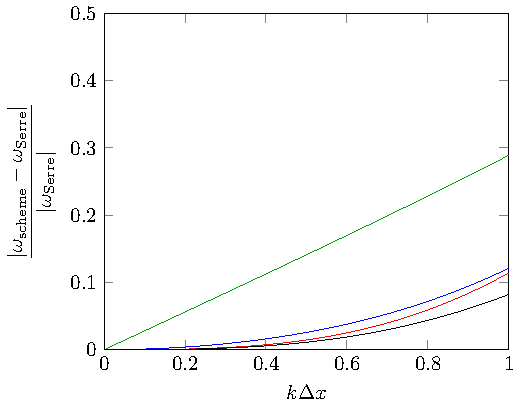
\includegraphics[width=\textwidth]{./chp5/figures/DispRelkh0p5.pdf}
		\subcaption*{\hspace{10 mm}$H = 1 $ and $k = 0.5$}
	\end{subfigure}%
	\begin{subfigure}{0.5\textwidth}
		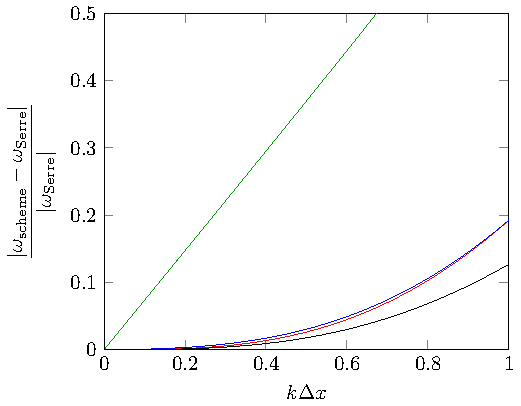
\includegraphics[width=\textwidth]{./chp5/figures/DispRelkh2p5.pdf}
		\subcaption*{\hspace{10 mm}$H = 1 $ and $k = 2.5$}
	\end{subfigure}
	\caption{Dipserion error for first-order FDVM ({\color{green!60!black} \solidrule}), second-order FDVM({\color{red} \solidrule}), second-order FEVM ({\color{blue} \solidrule})  and third-order FDVM ({\solidrule}).}
	\label{fig:DispErrMeth1}
\end{figure}

From these plots we can see that as expected as you increase the order of accuracy of the scheme your dispersion relation error decreases everywhere. This is most evident for the different order FDVM. Also we have as expected that increasing the resolution of our numerical methods decreases the dispersion error of the numerical scheme. 

More interesting is that the second-order FDVM performs better than the FEVM consistently across various numerical resolutions indicating that the FEVM will have a larger phase error than its FDVM counterpart. Thus it appears that error in approximating $\mathcal{G}$ was more significant than the error in approximating $\mathcal{R}^{\upsilon}$ for the dispersion relation.

Our results compare well with those of \cite{Filippini-etal-2016-381} who performed a similar analysis for their numerical method applied to the linearised Serre equations with $U=0$. We have extended their results by combining the spatial and temporal contribution to the dispersion relation and performing it on a different numerical method. 

These plots only depend on the parameter $kH$ and do not vary independently for $H$ or $k$. This parameter $kH$ is proportional to the shallowness parameter $\sigma$ with $2 \pi \sigma = kH $. So for $kH$ we have left shallow water and the Serre equations are no longer an appropriate model for water waves, although our results demonstrate that our numerical methods are still well approximating the dispersion relation of the Serre equations in this case. In general we also find that as $kH$ is increased our numerical methods perform worse generally although the dispersion relation still converges to $0$ as $\Delta x \rightarrow 0$. 

We will now turn our attention to demonstrating Von Neumann stability for the two finite difference methods described in this thesis [], and used for the purposes of comparison. We shall also see that we can use some of the previous working on the dispersion relation error to demonstrate stability for our FDVM and FEVM when $U=0$. 



\section{Von Neumann Stability}
To demonstrate Von Neumann stability we again begin with the linearised Serre equations \eqref{eqn:LinSerre} however will no longer require $U=0$, so we have

\begin{equation*}
	\frac{\partial  \eta}{\partial  t} + H\frac{\partial  \upsilon}{\partial  x} + U\frac{\partial  \eta}{\partial  x} = 0,
\end{equation*}
\begin{equation*}
	H\frac{\partial  \upsilon}{\partial  t} + gH\frac{\partial  \eta}{\partial  x} + UH\frac{\partial  \upsilon}{\partial  x} - \frac{H^3}{3}\left(U\frac{\partial^3  \upsilon}{\partial  x^3} + \frac{\partial^3  \upsilon}{\partial  x^3 \partial  t}  \right)  = 0.
\end{equation*}

As in the above dispersion relation analysis we will demonstrate the working for one problem and then just present the results for the other one to be both repeatable and brief. Our example will be the naive second-order finite difference method $\mathcal{D}$ \eqref{eq:Dnumdef}.

We will again begin by replacing both $\eta$ and $\upsilon$ by Fourier nodes \eqref{eqn:FourierNode}. Because our approximations to derivatives is constant for $\mathcal{D}$ we will provide all the factors for the second order centred finite difference approximations to derivatives of some quantity $q$ generated by making use of \eqref{eqn:fourierfactor}. Having all the factors associated with all the spatial derivatives we are really only left with the task of rearranging the equations and writing it in matrix form. The factors for each derivative approximation are

\begin{subequations}
	\begin{equation}
	\left(\frac{\partial q}{\partial x}\right)^n_j = \frac{- q^n_{j-1} + q^n_{j+1}}{2 \Delta x} = \frac{i \sin\left(k \Delta x\right)}{\Delta x} q^n_j
	\end{equation}
	
	\begin{equation}
\left(\frac{\partial^2 q}{\partial x^2}\right)^n_j = \frac{q^n_{j-1} - 2q^n_j + q^n_{j+1}}{\Delta x^2} = \frac{2 \cos\left(k \Delta x\right) - 2}{\Delta x^2} q^n_j 
	\end{equation}
	\begin{equation}
	\left(\frac{\partial^3 q}{\partial x^3}\right)^n_j = \frac{- q^n_{j-2}  + 2q^n_{j-1}  - 2q^n_{j+1} + q^n_{j+2}}{2\Delta x^3}=-4i\sin\left(k \Delta x\right)\frac{\sin^2\left(\frac{k \Delta x}{2}\right) }{\Delta x^3} q^n_j
	\end{equation}
	\label{eqn:FDfactorlist}
\end{subequations}

The numerical method $\mathcal{D}$ is just attained from replacing all the derivatives in \eqref{eqn:LinSerre} with the approximations in \eqref{eqn:FDfactorlist}. For the linearised equations the update formulas for $\mathcal{D}$ becomes

	\begin{equation*}
	\eta^{n+1}_j = \eta^{n-1}_j - \Delta t \left(U \frac{- \eta^{n}_{j-1} + \eta^{n}_{j+1} }{\Delta x} + H \frac{- \upsilon^{n}_{j-1} + \upsilon^{n}_{j+1}}{\Delta x}\right).
	\end{equation*}
	\begin{multline*}
	\upsilon^{n+1}_j - \frac{H^2}{3}\frac{\upsilon^{n+1}_{j-1} -2\upsilon^{n+1}_{j} +\upsilon^{n+1}_{j+1} }{\Delta x^2} 
	\\ =  \upsilon^{n-1}_j - \frac{H^2}{3}\frac{\upsilon^{n-1}_{j-1} -2\upsilon^{n-1}_{j} +\upsilon^{n-1}_{j+1}}{\Delta x^2}   \\+  \Delta t\left(- g\frac{-\eta^n_{j-1} + \eta^n_{j+1} }{\Delta x}   - U\frac{-\upsilon^n_{j-1} + \upsilon^n_{j+1} }{\Delta x} + \frac{H^2}{3}\left(U \frac{-\upsilon^{n}_{j-2} +2\upsilon^{n}_{j-1} -2\upsilon^{n}_{j+1} +\upsilon^{n}_{j+2}}{\Delta x^3}  \right)\right)  \\
	\end{multline*}


Since we have assumed that $\eta$ and $\upsilon$ are fourier nodes, we can just replace the finite difference approximations with the appropriate factors from \eqref{eqn:FDfactorlist}. After some rearranging we get that

\begin{equation*}
\eta^{n+1}_j = \eta^{n-1}_j - \Delta t \left(U  \frac{i \sin\left(k \Delta x\right)}{\Delta x}\eta^n_j + H\frac{i \sin\left(k \Delta x\right)}{\Delta x} \upsilon^n_j \right),
\end{equation*}
\begin{multline*}
\upsilon^{n+1}_j  =  \upsilon^{n-1}_j  -  \frac{3 \Delta x^2\Delta t}{3 \Delta x^2 -2{H^2} \left( \cos\left(k \Delta x\right) - 1 \right)}\bigg( g \frac{i \sin\left(k \Delta x\right)}{\Delta x}     \bigg) \eta^n_j\\ + U\frac{i \Delta t \sin\left(k \Delta x\right)}{\Delta x} \upsilon^n_j.  \\
\end{multline*}
 
We can rewrite this in matrix vector form as
\begin{equation}
\begin{bmatrix}
\eta^{n+1}_j \\
\upsilon^{n+1}_j\\
\eta^{n}_j \\
\upsilon^{n}_j
\end{bmatrix} = \matr{E}
\begin{bmatrix}
\eta^{n}_j \\
\upsilon^{n}_j\\
\eta^{n-1}_j \\
\upsilon^{n-1}_j
\end{bmatrix},
\end{equation}
where 
\begin{equation*}
\matr{E}_{\mathcal{D}} = \begin{bmatrix}
-  \dfrac{2 i\Delta t }{\Delta x} U\sin\left(k \Delta x\right)  & -  \dfrac{2 i\Delta t}{\Delta x} H \sin\left(k \Delta x\right)  & 1 &0 \\ \\
-\dfrac{6 gi \Delta x\Delta t}{3 \Delta x^2 -2{H^2} \left( \cos\left(k \Delta x\right) - 1 \right)}{ \sin\left(k \Delta x\right)}  & -\dfrac{2i \Delta t }{\Delta x} U \sin\left(k \Delta x\right)  & 0 &1 \\
1  & 0  &0 &0 \\
0  & 1  &0 &0 
\end{bmatrix} .
\end{equation*}

This is the evolution matrix $\matr{E}_{\mathcal{D}}$ and if its spectral radius is at most $1$ then $\mathcal{D}$ is stable.

After following through with the same process for $\mathcal{W}$ we get the following matrix equation

\begin{equation}
\begin{bmatrix}
\eta^{n+1}_j \\
\upsilon^{n+1}_j\\
\eta^n_j \\
\upsilon^n_j
\end{bmatrix}= \matr{E}_{\mathcal{W}}  \begin{bmatrix}
\eta^{n}_j \\
\upsilon^{n}_j\\
\eta^{n-1}_j \\
\upsilon^{n-1}_j
\end{bmatrix}.
\end{equation}
where
\begin{equation}
\matr{E}_{\mathcal{W}} = \begin{bmatrix}
{E}_{\mathcal{W}}^{0,0} & {E}_{\mathcal{W}}^{0,1} & 0 & - \dfrac{\Delta t}{\Delta x}H\frac{i\sin\left(k\Delta x\right)}{2} \\
-\dfrac{6 gi \Delta x\Delta t}{3 \Delta x^2 -2{H^2} \left( \cos\left(k \Delta x\right) - 1 \right)}{ \sin\left(k \Delta x\right)} & -\dfrac{2i \Delta t }{\Delta x} U \sin\left(k \Delta x\right)&0 & 1 \\
1&0&0&0\\
0&1&0&0
\end{bmatrix}
\end{equation}
with
\begin{align*}
&{E}_{\mathcal{W}}^{0,0} = 1 - \frac{\Delta t}{\Delta x}\left(-\dfrac{6 gi \Delta x\Delta t}{3 \Delta x^2 -2{H^2} \left( \cos\left(k \Delta x\right) - 1 \right)}{ \sin\left(k \Delta x\right)}\right)H\frac{i\sin\left(k\Delta x\right)}{2} \\ &- \frac{\Delta t}{\Delta x}U\left(\left(i\sin\left(k\Delta x\right)\right) - \frac{\Delta t}{\Delta x}U\left(\cos\left(k\Delta x\right) - 1\right)\right), \\
&{E}_{\mathcal{W}}^{0,1} = - \frac{\Delta t}{\Delta x} \left[H\frac{i\sin\left(k\Delta x\right)}{2}\left( 1 -\dfrac{2i \Delta t }{\Delta x} U \sin\left(k \Delta x\right) \right)   -U\left(\frac{\Delta t}{\Delta x}H\left(\cos\left(k\Delta x\right) - 1\right)\right) \right].
\end{align*}


If the evolution matrix $\matr{E}_{\mathcal{W}}$ has a spectral radius less than or equal to $1$ then $\mathcal{W}$ is stable.

It can be seen that we generated this evolution matrix for each of the FDVM and FEVM. In particular we have that

\begin{align*}
&\matr{E}_{1} = \matr{I} - \Delta t \matr{F}_1 \\
&\matr{E}_{FD2} = \matr{I} - \Delta t \matr{F}_{FD2} + \frac{1}{2} \Delta t^2 \matr{F}_{FD2}^2 \\
&\matr{E}_{FEM2} =  \matr{I} - \Delta t \matr{F}_{FEM2} + \frac{1}{2} \Delta t^2 \matr{F}_{FEM2}^2\\
&\matr{E}_{3} = \matr{I} - \Delta t \matr{F}_{3} + \frac{1}{2} \Delta t^2 \matr{F}_3^2 - \frac{1}{6} \Delta t^3 \matr{F}_3^3. \\
\end{align*}

For the FDVM and FEVM the matrix equation is a bit simpler

\begin{equation}
\begin{bmatrix}
\eta \\
\upsilon\\
\end{bmatrix}^{n+1}_j = \matr{E}  \begin{bmatrix}
\eta\\
\upsilon\
\end{bmatrix}^{n}_j .
\end{equation}
As with the finite difference methods if the spectral radius of the evolution matrix is at most $1$ then the scheme is stable.

We will now present the results of our analysis of the stability of all these methods for various $U$, $H$ and $k$ values. 

\subsection{Results}
We will demonstrate that these finite difference methods possess Von Neumann stability numerically. We do this by calculating the spectral radius of the growth matrices numerically for various fixed $H$ and $k$ values and demonstrate the behaviour of this spectral radius as $\Delta x$ changes. We use the CFL condition to determine $\Delta t$ given $\Delta x$, and in particular we again have $\Delta t =   \left( 0.5 / \sqrt{gH} \right) {\Delta x} $. We first show the results for $U = 0$ so that we  can demonstrate the stability of the FDVM and FEVM as well and then allow various $U$ values and we therefore do not include the FDVM and FEVM.

\subsubsection{Quiescent Fluid}
This is the situation in which we are most interested in for the purposes of ocean modelling. Most of the numerical experiments we perform later will occur in this region where the water is still with waves propagating on top. This is also the scenario in which the growth matrices for the FDVM and FEVM was calculated and thus we can only demonstrate the stability of all methods in this region. Although of course as mentioned previously the FDVM and FEVM inherit their stability from the FVM at their core.

The spectral radius for a range of $\Delta x$ values were plotted in Figure~\ref{fig:Stabu=0} for all numerical methods in this thesis. The representative values of $kH =0.5$ and $kH = 2.5$ were the chosen due to their use in the dispersion error analysis for the stability results plotted in Figure~\ref{fig:DispErrMeth1}.

Our results demonstrate that all numerical methods satisfy the stability condition for a range of $kH$ values with $U=0$ as all methods have growth matrices with spectral radius less than or equal to $1$. Indeed this is what we found generally for all these methods for other values of $hK$ as well.

We note that both the second-order FDVM ({\color{red} \solidrule}) and FEVM ({\color{blue} \solidrule}) have very similar spectral radius values such that their plots overlap and only the curve for the FEVM ({\color{blue} \solidrule}) is visible. We also observe similar behaviour for the two second-order finite difference methods $\mathcal{D}$ ({\color{violet!80!white} \solidrule}) and $\mathcal{W}$ ({\color{orange} \solidrule}) so that only the curve for $\mathcal{W}$ ({\color{orange} \solidrule}) is visible.

We observe that the spectral radius for the second-order finite difference methods $\mathcal{D}$ and $\mathcal{W}$ are consistently $1$ when $U=0$ for various $hK$ and $
k\Delta x$ values. This can be seen in Table~\ref{tab:Averageofspectralradiusu=0}, where the average of the spectral radius for $\mathcal{D}$ and $\mathcal{D}$ over various $k \Delta x$ values is $1$ plus a number which is just round-off errors accumulated by doing this process numerically.

\begin{figure}
	\centering
	\begin{subfigure}{0.5\textwidth}
		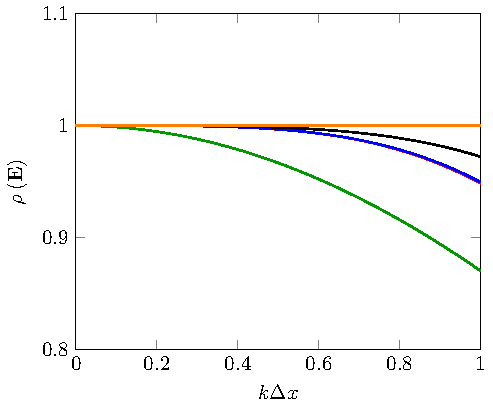
\includegraphics[width=\textwidth]{./chp5/figures/stabilityu=0kh0p5.pdf}
		\subcaption*{\hspace{10 mm}$U =0$, $H = 1 $ and $k = 0.5$}
	\end{subfigure}%
	\begin{subfigure}{0.5\textwidth}
		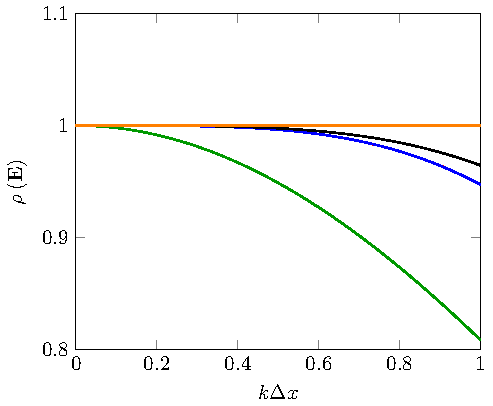
\includegraphics[width=\textwidth]{./chp5/figures/stabilityu=0kh2p5.pdf}
		\subcaption*{\hspace{10 mm}$U =0$, $H = 1 $ and $k = 2.5$}
	\end{subfigure}
	\caption{Spectral radius of growth matrix $\matr{E}$ for first-order FDVM ({\color{green!60!black} \solidrule}), second-order FDVM({\color{red} \solidrule}), second-order FEVM ({\color{blue} \solidrule}), third-order FDVM ({\solidrule}), $\mathcal{D}$ ({\color{violet!80!white} \solidrule}) and $\mathcal{W}$ ({\color{orange} \solidrule}) .}
	\label{fig:Stabu=0}
\end{figure}

\begin{table}
	\centering
	\begin{tabular}{l  c  c}
		Method & $kH$& Average\\
		\hline && \\
		$\mathcal{D}$& $0.5$ & $1+ 4\times 10^{-16}$  \\
		$\mathcal{D}$& $2.5$ & $1+ 4\times 10^{-16}$  \\
		\hline \\
		$\mathcal{W}$& $0.5$ & $1+ 4\times 10^{-16}$  \\
		$\mathcal{W}$& $2.5$ & $1+ 4\times 10^{-16}$ 
	\end{tabular}
	\caption{Average of $\rho\left(\matr{E}\right)$ over all $\Delta x$ values for the second-order finite difference methods when $U=0$.}
	\label{tab:Averageofspectralradiusu=0}
\end{table}


\subsubsection{Non-zero Mean Flow} 
The situation of waves on still water is certainly the most common situation in ocean modelling, however there are scenarios that can arise where certain regions have a mean flow and we are interested in the waves on top, such as undular bores. Therefore we must also demonstrate stability in this case fo the two finite difference methods. Since the dispersion relation analysis that derived the evolution matrix for the FDVM and FEVM assumed $U=0$ we do not demonstrate their stability here. 

We have investigated the behaviour of the spectral radius of the growth matrix for various values of $U$, $kH$ and $\Delta x$. We present the results for $U =1$ with $kH =0.5$ and $2.5$ in Figure~\ref{fig:Stabu=1}. These values were chosen because they are representative of the behaviour for both methods for most values of $U$ and $kH$, and because they match the previous values in the results[]. 

These results demonstrate that the naive second-order method $\mathcal{D}$ is still stable even with a background mean flow, with a spectral radius that is consistently $1$. This is demonstrated in Table~\ref{tab:Averageofspectralradiusu=1} as well where the average spectral radius is $1$ plus a number that is at round-off error. This behaviour was consistent for various $U$, $kH$ and $\Delta x$ values provided the CFL condition was used to determine $\Delta t$. Therefore this method is stable as desired for a range of flow scenarios. 

Unfortunately the Lax-Wendroff finite difference method $\mathcal{W}$ is no longer stable anywhere with growth factors that are consistently larger than $1$ although it approaches stability as $\Delta x \rightarrow 0$. This is evident in Table \ref{tab:Averageofspectralradiusu=1} where the average spectral radius is larger than $1$ by significantly more than round-off error. By modifying the parameters we can increase the spectral radius as desired. However, the parameters do not follow some simple rule and their behaviour is quite complicated, it is however that case that our largest $\Delta x$ value did correspond to our largest spectral radius. However, the interaction between the spectral radius, $hK$ and $U$ is not so obvious. Since the spectral radius was consistently larger than $1$ when $U \neq 0$ this means the Lax-Wendroff method is not stable unless $U=0$. Although the growth factors are still very close to $1$ for most situations and so the instabilities may not be apparent when performing numerical experiments, as we demonstrate in chapter []. 
\begin{figure}
	\centering
	\begin{subfigure}{0.5\textwidth}
		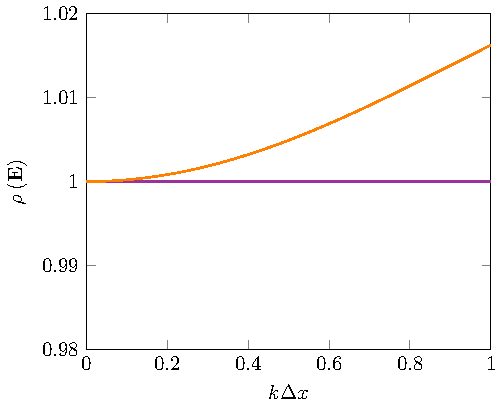
\includegraphics[width=\textwidth]{./chp5/figures/stabilityu=1kh0p5.pdf}
		\subcaption*{\hspace{10 mm}$U =1$, $H = 1 $ and $k = 0.5$}
	\end{subfigure}%
	\begin{subfigure}{0.5\textwidth}
		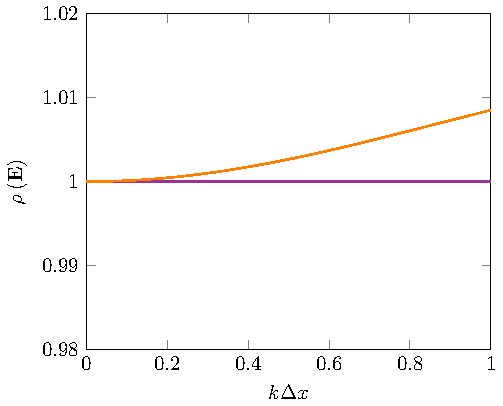
\includegraphics[width=\textwidth]{./chp5/figures/stabilityu=1kh2p5.pdf}
		\subcaption*{\hspace{10 mm}$U =1$, $H = 1 $ and $k = 2.5$}
	\end{subfigure}
	\caption{Spectral radius of growth matrix $\matr{E}$ for $\mathcal{D}$ ({\color{violet!80!white} \solidrule}) and $\mathcal{W}$ ({\color{orange} \solidrule}) .}
	\label{fig:Stabu=1}
\end{figure}


\begin{table}
	\centering
	\begin{tabular}{l  c  c}
		Method & $kH$& Average\\
		\hline && \\
		$\mathcal{D}$ & $0.5$ & $1+ 4\times 10^{-16}$  \\
		$\mathcal{D}$ & $2.5$ & $1+ 4\times 10^{-16}$  \\
		\hline \\
		$\mathcal{W}$ & $0.5$ & $1+ 6\times 10^{-3}$  \\
		$\mathcal{W}$ & $2.5$ & $1+ 3\times 10^{-3}$   \\
	\end{tabular}
	\caption{Average of $\rho\left(\matr{E}\right)$ over all $\Delta x$ values for the second-order finite difference methods when $U=1$.}
	\label{tab:Averageofspectralradiusu=1}
\end{table}